\documentclass[a4paper]{article}

%% Language and font encodings
\usepackage[english]{babel}
\usepackage[utf8x]{inputenc}
\usepackage[T1]{fontenc}
\usepackage{pdfpages}
\usepackage{booktabs}
\usepackage{fancyhdr}
\usepackage{lastpage}
\usepackage{siunitx}
\usepackage{array,longtable}
%\usepackage{geometry}
\renewcommand*{\arraystretch}{1.5}

%% Sets page size and margins
\usepackage[a4paper,top=3cm,bottom=2cm,left=2cm,right=2cm,marginparwidth=1.75cm]{geometry}

%% Useful packages
\usepackage{amsmath}
\usepackage{graphicx}
\usepackage[UKenglish]{datetime}
\usepackage[colorinlistoftodos]{todonotes}
\usepackage[colorlinks=true, allcolors=black]{hyperref}
\usepackage{enumitem}
\pagestyle{fancy}
\fancyhf{}
\lhead{British Science Week | 12th - 14th March 2019}
\rhead{Version 2.0 | Release\\Updated: \currenttime \ \today}
\rfoot{Page \thepage\ of \pageref{LastPage}}

\title{British Science Week\\12th - 14th March 2019\\Information for Helpers}
%\author{Tomos Fearn\\tof7@aber.ac.uk}
\date{}

\begin{document}
\long\def\/*#1*/{}
\maketitle
%\newpage
%\tableofcontents
%\newpage

\noindent
Thank you for offering to help during Science Week this week. The following information is useful for helpers from Aber Robotics Club, CompSci, Physics and Maths.

\section*{Setup}
Setup will commence Monday afternoon 11th March at 12:10. We will be meeting in the Physics part 1 lab (MP 1.00), to collect the exhibits and move everything via trailer to the sports cage. We will need to be finished by 17:30.

\section*{Take-down}
Taking down the exhibits commences on Thursday 15:00 at the sports cage. We will be moving everything back to the Physical Sciences building via trailer/van.

\section*{Social Media}
If you are posting on social media about science week please make sure you do the following:
\begin{itemize}[nolistsep]
	\item Don't post pictures with children in them - permission from parents is needed (which we can't get). Focus on the stand instead.
	\item Ensure you tag CWPSI - \textbf{\texttt{@AberUniCWPSI}} use the hashtag \textbf{\texttt{\#BSW19}} - CWPSI will then retweet.
	\item British Science Week can be tagged as \textbf{\texttt{@ScienceWeekUK}}
\end{itemize}

\section*{Times}
\begin{center}
\begin{tabular}{ |c|c|c| } 
\hline
Day & Day Time & Evening \\
\hline
\hline
Tuesday & 8:30 - 16:00 &  \\ 
\hline
Wednesday & 8:30 - 15:00 & 16:00 - 18:30 \\ 
\hline
Thursday & 8:30 - 15:00 & 15:00 - 18:00 \\ 
\hline
\end{tabular}
\end{center}

\section*{Timesheet}
You can access the timesheet of helpers at the Doodle poll https://doodle.com/poll/he8uu7p9xgxg7eyp


\section*{Information from CWPSI}
\subsection*{Refreshments}
``We will provide (free) DIY tea / coffee etc on the Balcony (at the Counter area); please BRING A MUG/ beaker if possible to save on wasteful paper cups – we only have a few for teachers etc.   Ask a CWPSI team member if supplies run out or you need particular items.  Try and refill the kettles as you go, so the next person doesn’t have a long wait.  Please try and keep the area tidy / clean and take care – HOT drinks and SMALL people do not mix well!'' - CWPSI

\subsection*{Lunch and Water}
``For those on stands all day – or working over the lunchtime – we will provide an honour system for food as in previous years.  Please respect this: we can only continue to provide this is if you are fair and have one of each item. We have based the numbers on the info on your forms. Lunch will be out from approx. 12 in the changing room on the Balcony.  There will be crisps, fruit, a sweet item and a (labelled) bread roll.  We will NOT BE PROVIDING WATER BOTTLES at lunchtime - use your own water bottle or mug (for the sake of the planet!).'' - CWPSI

\subsection*{Yellow Tent}
``We use this for lost small people – or those who need a quiet space. SO if there are lost children please send them there / accompany them and alert a CWPSI team member.  If you see rowdy older children using it to chill can you help monitor and ask them to ‘move on’. '' - CWPSI

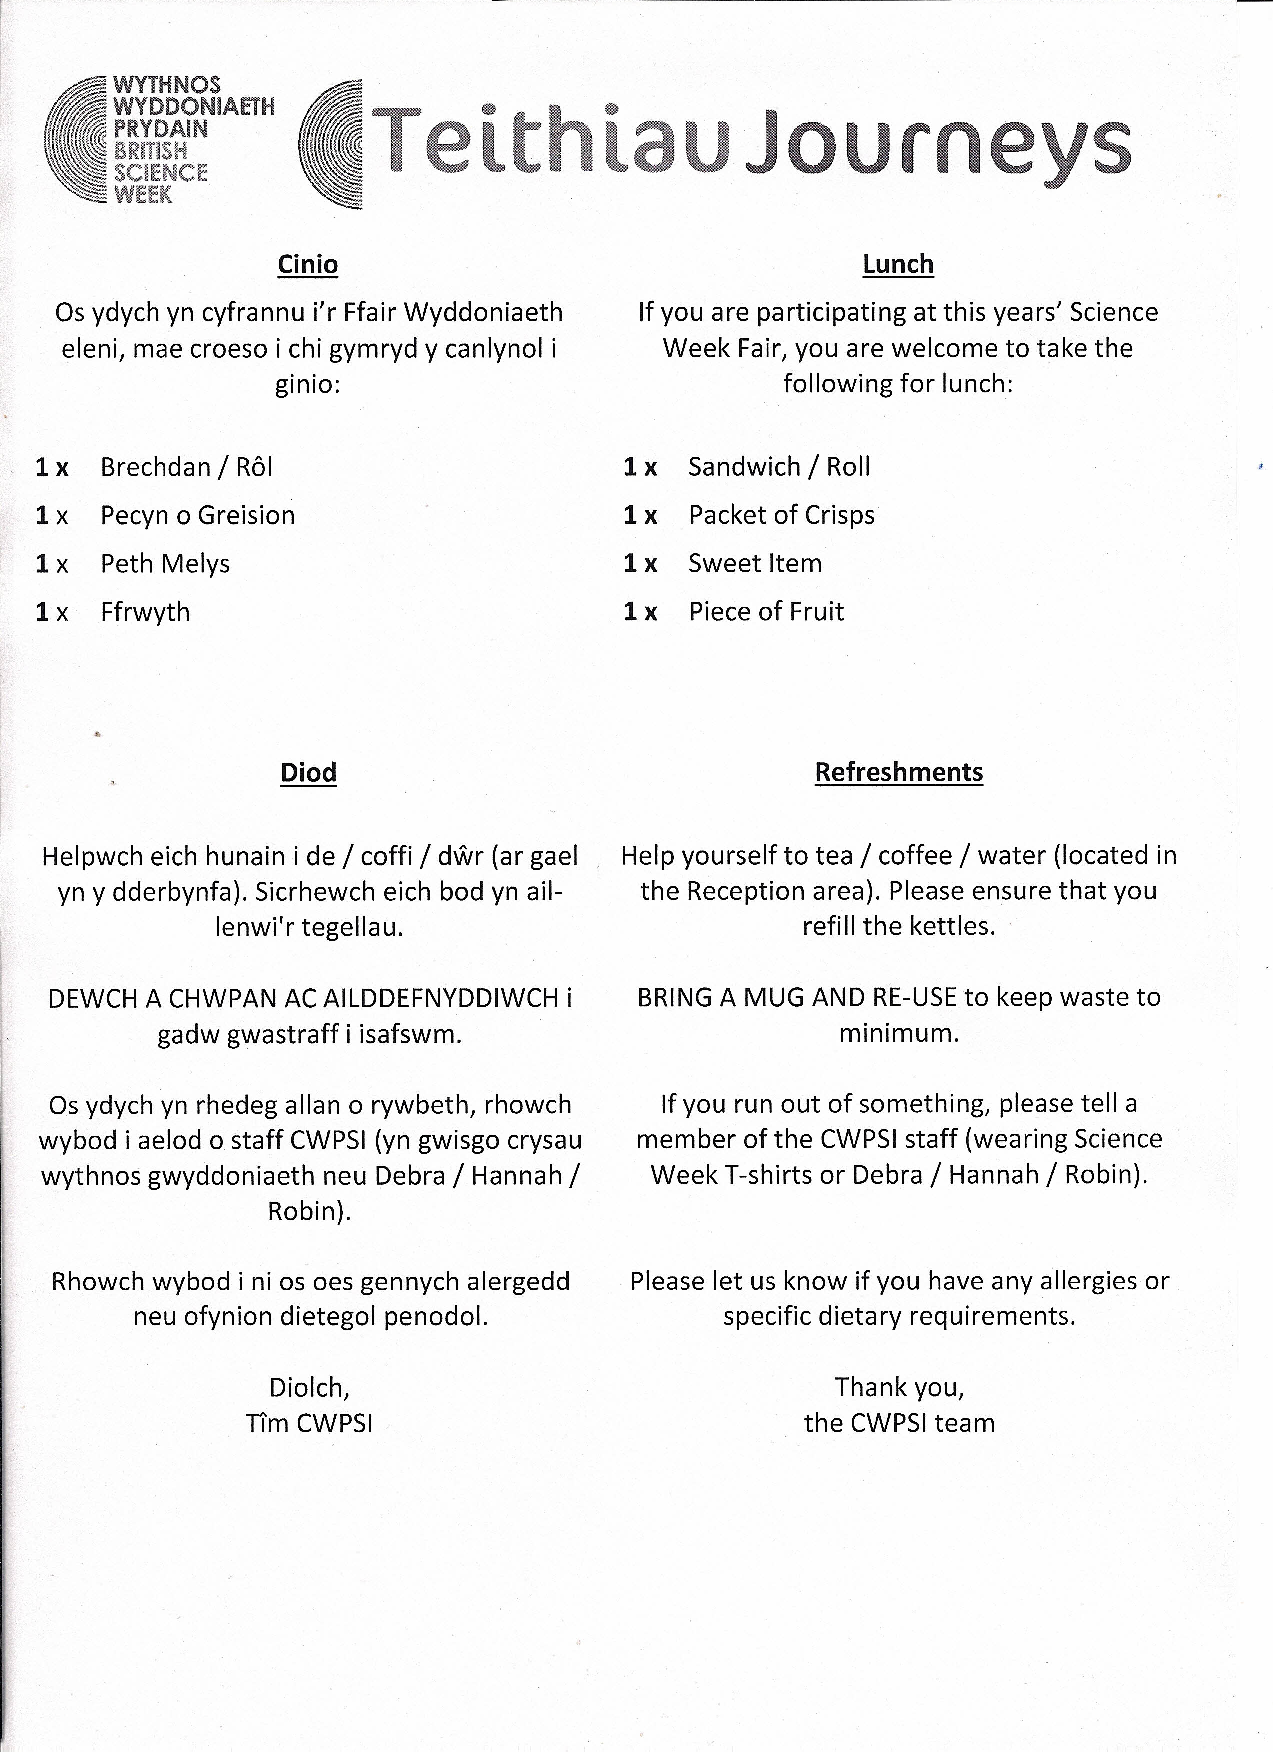
\includepdf[pages=-]{refreshments.pdf}
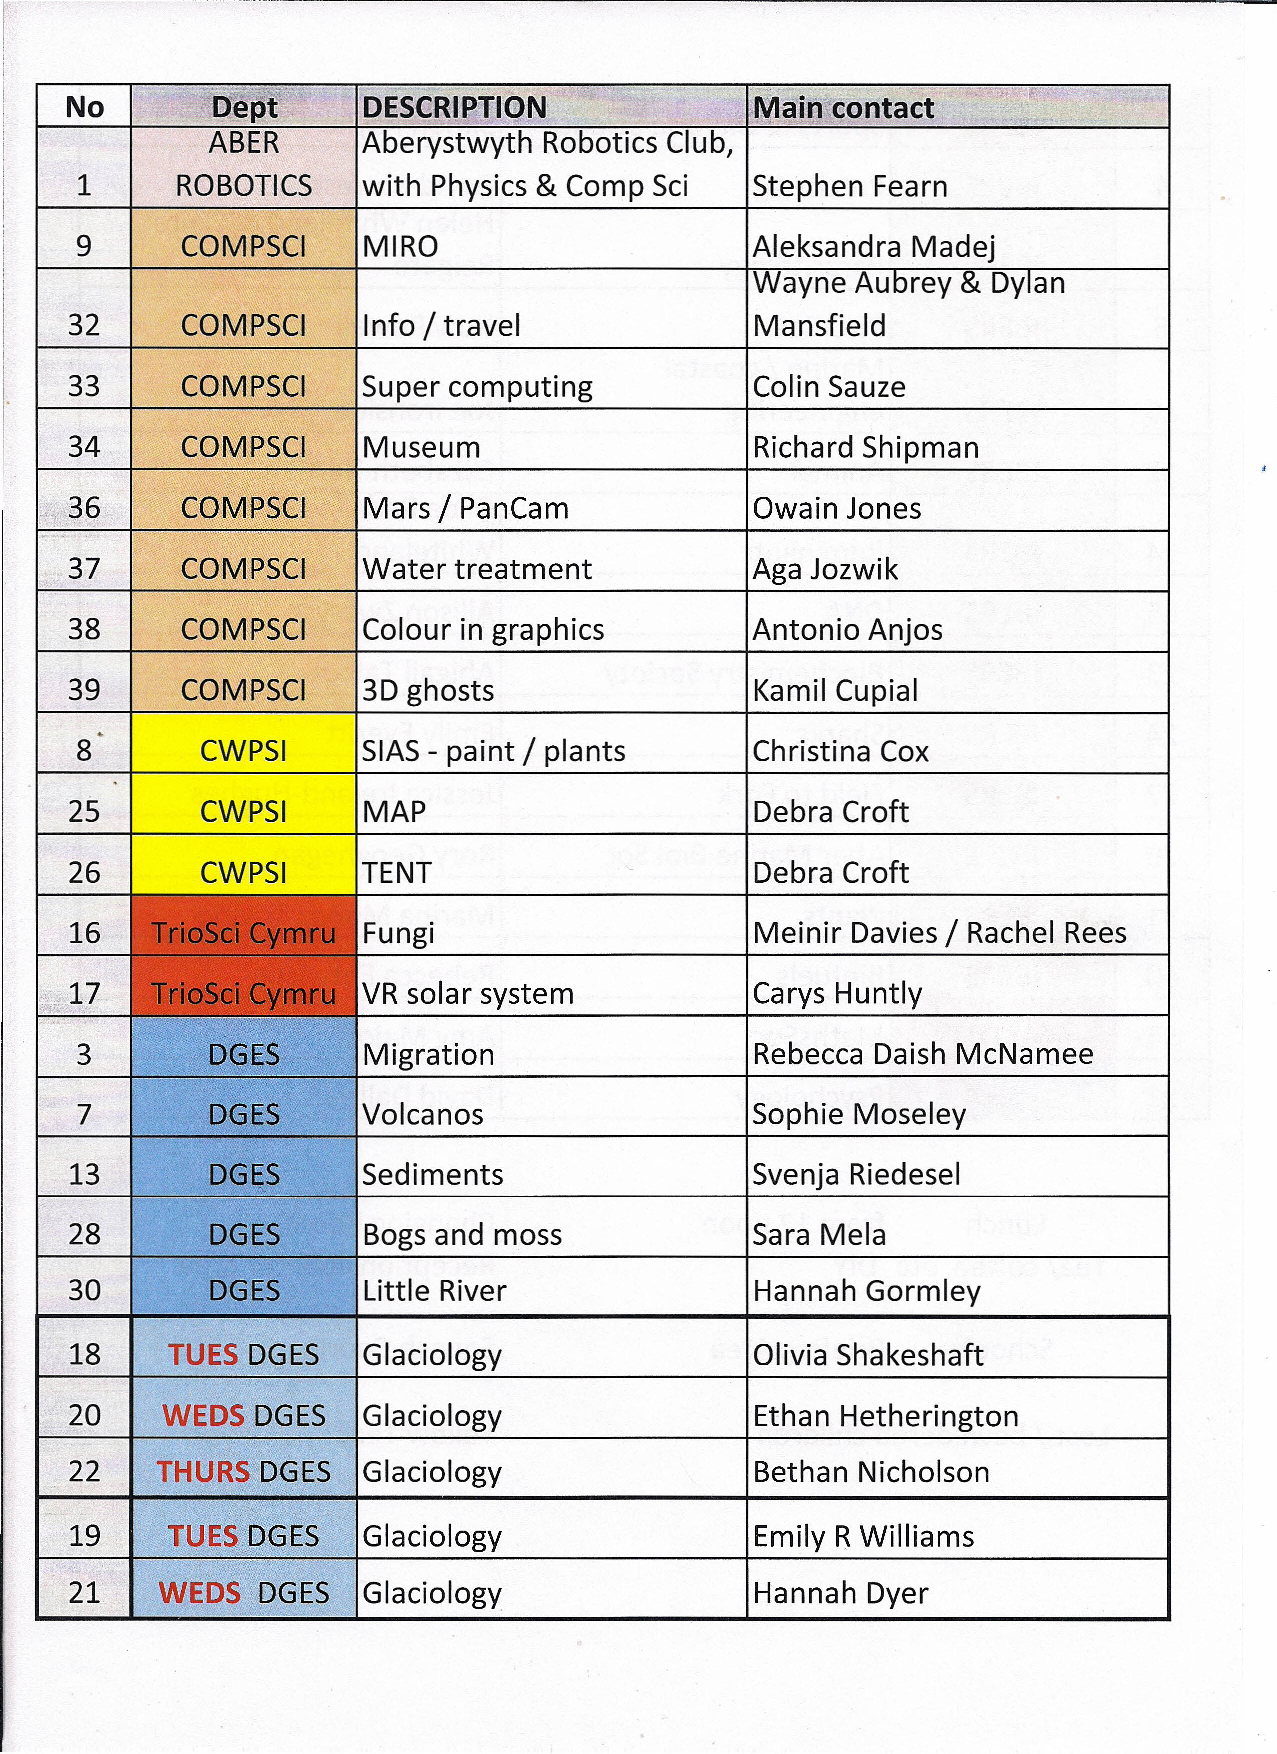
\includepdf[pages=-]{stands.pdf}
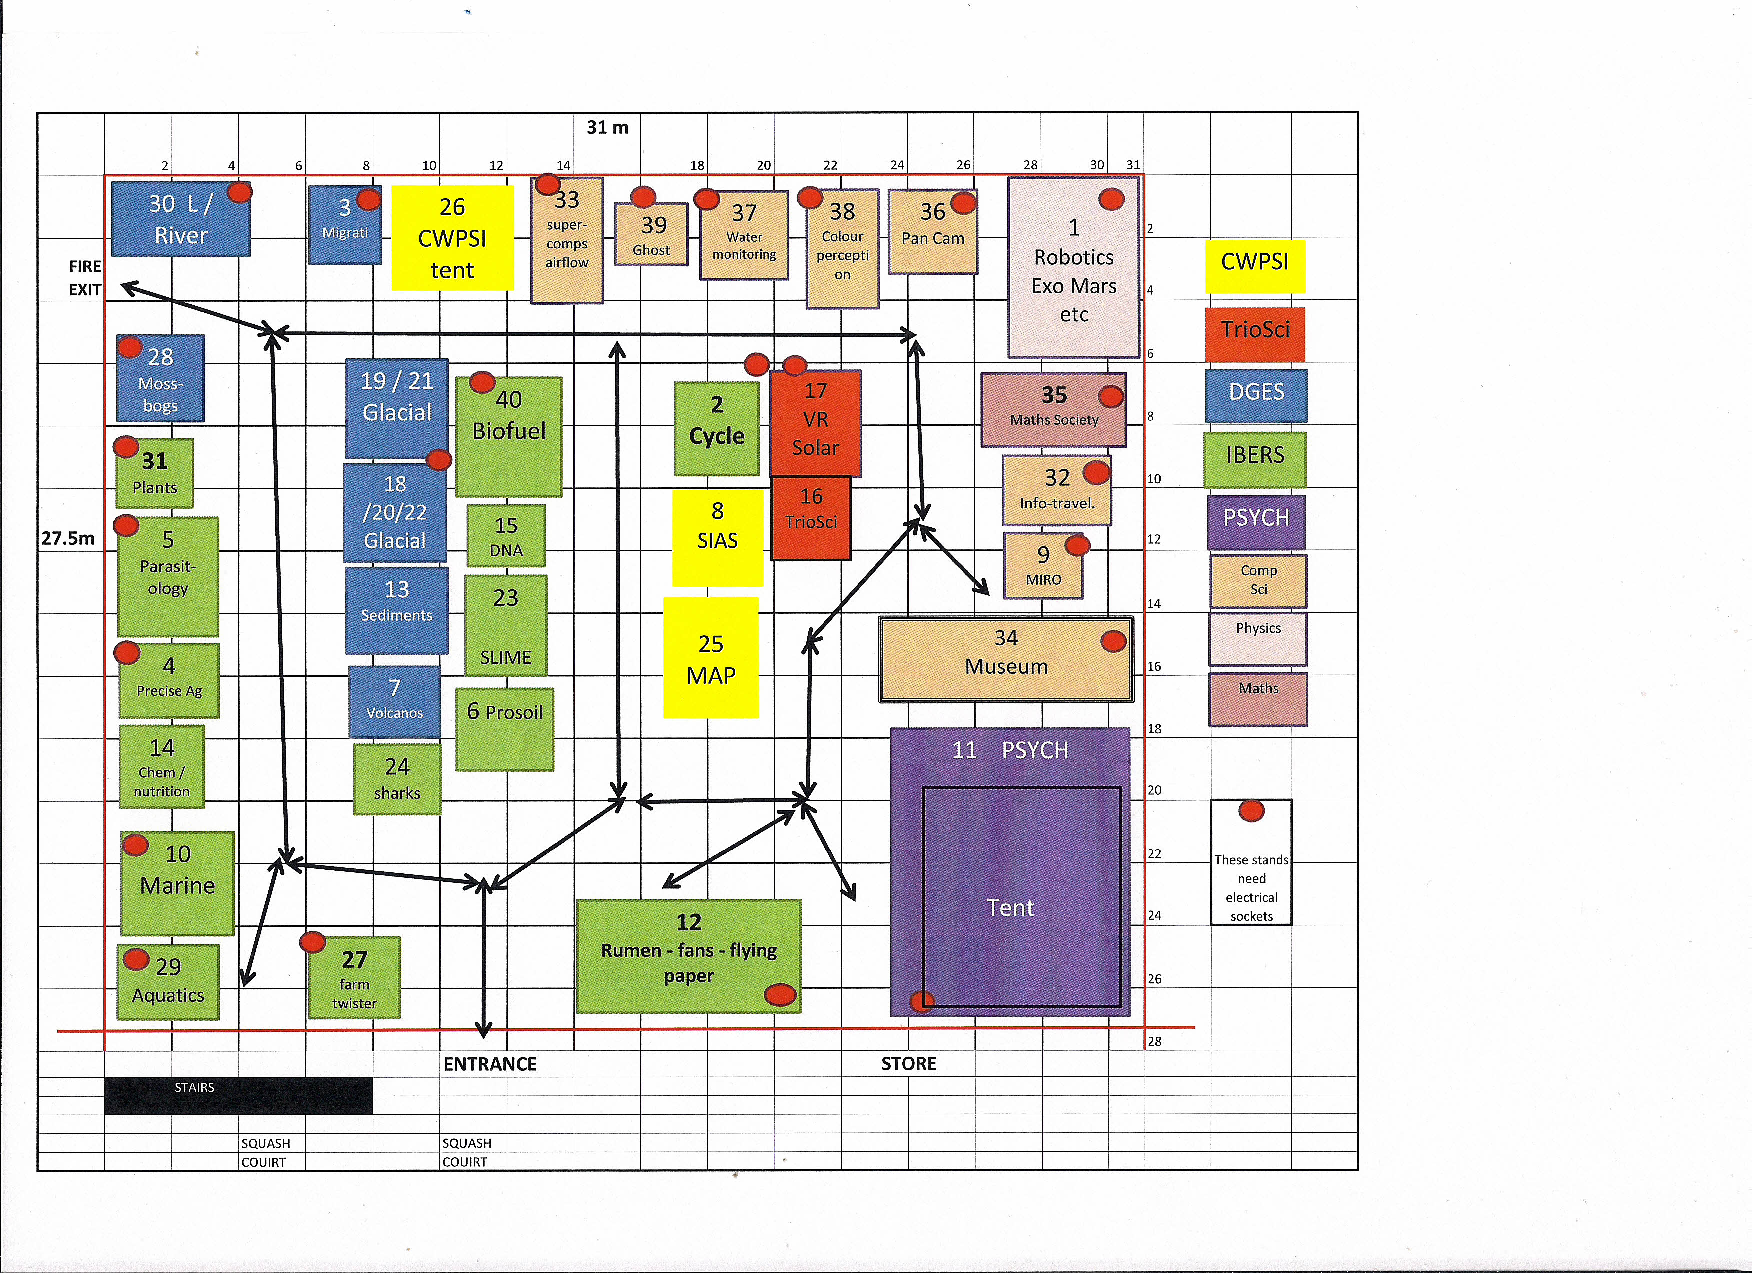
\includepdf[pages=-]{map.pdf}

\newpage
\section*{List of Exhibits}
\begin{center}
\begin{tabular}{ |c|c| } 
\hline
Name & Location \\
\hline
\hline
VR (Vive and PC) & MP 1.04 \\ 
\hline
Gazebo & TBC \\
\hline
Valiants & MP 1.05 \\
\hline
Magician Chassis & MP 1.05 \\
\hline
Pioneer & Tomos \\
\hline
Tango & MP 1.05 \\
\hline
Sherbert Lemon & MP 1.05 \\
\hline
Barnes & Compsci Van \\
\hline
Mini-Barnes & MP 1.00 \\
\hline
Mars Terrain & Basement \\
\hline
Sensor Board & Physics Museum \\
\hline
UAV & MP 1.05 \\
\hline
Spider & MP 1.00 \\
\hline
TurtleBot & MP 1.05 \\
\hline
Humanoid & MP 1.05 \\
\hline
Blackbot & MP 1.05 \\
\hline
Red Driverless Car & MP 1.05 \\
\hline
Black Driverless Car & MP 1.00 \\
\hline
Handles 1 + 2 & MP 1.00 \\
\hline
Scutter & MP 1.00 \\
\hline 
TweedleDum & MP 1.00 \\
\hline
Boat & MP 1.00 \\
\hline
Lego NXT (w. tablets) & MP 1.05 \\
\hline
\end{tabular}
\end{center}

\section*{Other stuff to take}
\begin{center}
\begin{tabular}{ |c|c| } 
\hline
Name & Location \\
\hline
\hline
Risk Assessment & Steve \\ 
\hline
Green Dist Box & MP 1.05 \\ 
\hline
Big Maze (w.corner pieces) & MP 1.05 + MP 1.00 \\ 
\hline
Popup banner & MP 1.05 \\
\hline
Stickers & MP 1.05 \\
\hline
Posters and boards & MP 1.05 \\
\hline
Velcro, pins and duct tape & MP 1.00 \\
\hline
Tripods x2 (for VR) & Steve \\
\hline 
\end{tabular}
\end{center}

\section*{Document Version}
V2.0 Release | Added info from pack | \currenttime \ \today \newline
V1.0 Release | Sent to helpers | 13:41 Sunday 10th March, 2019

\end{document}
